\documentclass[10pt,twocolumn,letterpaper]{article}

\usepackage{cvpr}
\usepackage{times}
\usepackage{epsfig}
\usepackage{graphicx}
\usepackage{cite}
\usepackage{amsmath}
\usepackage{amssymb}

% Include other packages here, before hyperref.

% If you comment hyperref and then uncomment it, you should delete
% egpaper.aux before re-running latex.  (Or just hit 'q' on the first latex
% run, let it finish, and you should be clear).
\usepackage[breaklinks=true,bookmarks=false]{hyperref}

\cvprfinalcopy % *** Uncomment this line for the final submission

\def\cvprPaperID{****} % *** Enter the CVPR Paper ID here
\def\httilde{\mbox{\tt\raisebox{-.5ex}{\symbol{126}}}}

% Pages are numbered in submission mode, and unnumbered in camera-ready
%\ifcvprfinal\pagestyle{empty}\fi
%\setcounter{page}{2571}
\begin{document}

%%%%%%%%% TITLE
\title{	CNN Based Image Classification}

\author{Xiaoling Long\\
SIST\\
ShanghaiTech Univ.\\
{\tt\small longxl@shanghaitech.edu.cn}
% For a paper whose authors are all at the same institution,
% omit the following lines up until the closing ``}''.
% Additional authors and addresses can be added with ``\and'',
% just like the second author.
% To save space, use either the email address or home page, not both
\and
Hongyu Chen\\
SIST\\
ShanghaiTech Univ.\\
{\tt\small chenhy3@shanghaitech.edu.cn}
\and
Ruiqi Luo\\
SIST\\
ShanghaiTech Univ.\\
{\tt\small luorq@shanghaitech.edu.cn}
}


\maketitle
%\thispagestyle{empty}

%%%%%%%%% ABSTRACT
\begin{abstract}
   The convolution networks make a great success in image classification since AlexNet proposed for classification in ImageNet chanllenge. This End-to-End training method make researcher focus more on how to build an efficient network. The user focus more on how to use convolution networks in their application. After AlexNet, there are many ConvNet architecture proposed, such as VGGNet  and ResNet. These ConvNet architectures are widely  used in many actual real applications.
\end{abstract}

%%%%%%%%% BODY TEXT
\section{Introduction}
Image classification is a fundamental challenge in computer vision\cite{felzenszwalb2013visual}. Consider the problem of detecting objects from a category, such as people or cars, in static images. This is a difficult problem because objects in each category can vary greatly in appearance. Variations arise from changes in illumination, viewpoint, and intra-class variability of shape and other visual properties among object instances. For example, people wear different clothes and take a variety of poses while cars come in various shapes and colors.Classification   between   the   objects   is   easy   task   for  humans  but  it  has  proved  to  be  a  complex  problem for machines.Image classification refers to the labeling of images into one of a number of predefined categories.
Image classification is an important and challenging task in various application domains, including biomedical imaging, biometry, video surveillance, vehicle navigation, industrial visual inspection, robot navigation, and remote sensing \cite{kamavisdar2013survey}.

Image classification uses both supervised and unsupervised
Traditional  methods  of  computer  vision  and  machine
learning cannot match human performance on tasks such
as the recognition of handwritten digits or traffic signs.\cite{ciregancolumn}

Non‐parametric  classifiers  such  as  decision tree   classifier,  neural   network,   SVM   classifier and knowledge based classification are also very common in image classification.

Disadvantages about the deep learning.For the deep learning based algorithm required the ability of labeled samples for training. The collection of labeled data is a time consuming process as well as costly.


%-------------------------------------------------------------------------
\section{Evaluation standard}
Two method are commons used for the image classification one is TOP 1 error another is TOP 5 error.
TOP 1 error: The correct answer is the top guess.TOP 5 error: The correct answer is in the top-5 guess


\section{Dataset}


There are several common dataset for the image classification.such as the MINIST dataset\cite{lecun1998gradientbased},ImageNet\cite{russakovsky2015imagenet} 
COCO dataset \cite{lin2014microsoft}.PASCAL\cite{pascal-voc-2012} CIFAR\cite{Krizhevsky2009Learning}and the Open Image which is from google.

MNIST is a hand-written digital database with 60,000 training sample sets and 10,000 test sample sets. Each sample image has a height of 28*28.This dataset is stored in binary and cannot be viewed directly in image format, but it is easy to find tools to convert it to image format.

 ImageNet is an image dataset organized according to the WordNet hierarchy. Each meaningful concept in WordNet, possibly described by multiple words or word phrases, is called a "synonym set" or "synset". There are more than 100,000 synsets in WordNet, majority of them are nouns (80,000+).


COCO is a large-scale object detection, segmentation, and captioning dataset. COCO has several features:Object segmentation,Recognition in context
Superpixel stuff segmentation,
330K images ($>$200K labeled),
1.5 million object instances,
80 object categories,
91 stuff categories,
5 captions per image,
250,000 people with keypoints.


The main goal of this challenge is to recognize objects from a number of visual object classes in realistic scenes (i.e. not pre-segmented objects). It is fundamentally a supervised learning learning problem in that a training set of labelled images is provided. The twenty object classes that have been selected are: 

Typical CIFAR daset contains  the  CIFAR-10 dataset ,he CIFAR-10 dataset consists of 60000 32x32 colour images in 10 classes, with 6000 images per class. There are 50000 training images and 10000 test images.

The dataset is divided into five training batches and one test batch, each with 10000 images. The test batch contains exactly 1000 randomly-selected images from each class. The training batches contain the remaining images in random order, but some training batches may contain more images from one class than another. Between them, the training batches contain exactly 5000 images from each class.
CIFAR-100 dataset
This dataset is just like the CIFAR-10, except it has 100 classes containing 600 images each. There are 500 training images and 100 testing images per class. The 100 classes in the CIFAR-100 are grouped into 20 superclasses. Each image comes with a "fine" label (the class to which it belongs) and a "coarse" label (the superclass to which it belongs).

Open Image is a data set that contains ~9 million image URLs. The images are divided into more than 6000 categories by tag annotations. The tags in the dataset contain more real-life entities than ImageNet (1000), which is enough for us to train deep neural networks from scratch.


\section{CNN Based Image classification}

\par
The ImageNet Large Scale Visual Recognition Challenge(ILSRC) is a benchmark in object category classification and detection on $1000$-classes and millions of images. After AlexNet achieved hugu success in ILSRC-2012, there are various variations of AlexNet\cite{krizhevsky2012imagenet} and many other types of ConvNet for image classification. Since that, ConvNet is widely used for image classification. \cite{aloysius2017review} illustrate beriefly what is ConvNet, the components of ConvNet, the activation function in ConvNet, from LeNet to ResNet bunch of successful ConvNet and some open issues on CNN based image classification. LeNet is first proposed CNN based image classifition method.

\par
LeNet\cite{lecun1990handwritten} \cite{leou11comparison} is first proposed CNN based image classifition method. After that, AlexNet\cite{krizhevsky2012imagenet} brought Convolutional neural network into ILSRC. In this implementation, it contains 8 layers \- 5 convolutional and 3 fully-conneted. The main features of this network's architecture are ReLU\cite{nair2010rectified} as activation function, overlapping pooling and skills for reducing overfitting. Based on ReLU and overlapping pooling, the network err rate has more or less reduction, and ReLU network learn several times faster than other saturating acitvation function such as tanh neurons network. Overfitting is common issue for machine learning, it uses data augmentation and dropout to avoid overfit. Dropout is a skill to reduce argument or increase hypothesis. There are many discuss about this. As to data augmentation, it enlarge the dataset by cropping $224\times 224$ patched from the original image as well as these patchs' horizontal refliction. At the end averaging the predications as final socre.
\par
\cite{donahue2014decaf} explored the generalization ability of ConvNet features, releasing DeCAF. Traditional image classifition pipeline is extracting feature, building bag of feature then put into classifier. \cite{zeiler2011adaptive} propose a CNN based feature extractor. This is an unsurpervising learning ConvNet or in other words, input image is also the kind of ground truth. After feature extracting, the final result can classify by any classifier. This strategy is used as a tool for visualizing and undestanding how ConvNet works \cite{zeiler2014visualizing}.ConvNet have an impressive classification performance. However there is no clear understanding for why this work. \cite{zeiler2014visualizing} propose a architecture for visualizing and undestanding how ConvNet works.
\par
OverFeat\cite{sermanet2013overfeat} is a integrated recognition, localization and detection. This network uses CNN extract feature from image and then perform classification and localization and detection. Multi-scale classification brought up in \cite{sermanet2013overfeat} to increase accuracy.
\par
``Networ In Network"\cite{lin2013network} propsed a new deep network structure. Different from conventional convolution layer, it brings up a new Mlpconv layer. This Mlpconv layer consist of sliding multilayer perceptron(MLP) window. In stead of fully-connected layer at the top of network, global average pooling is used to produce the resulting vector fed directly into the softmax layer. Verified by experiments, this NIN structure indeed works well on some benchmark datasets, and global average pooling can be regarded as regularizer. THis glolbal average pooling has no parameter. This stratety is used widely afterwards. $1\times 1$ convolution conception proposed in \cite{lin2013network} is used in GoogLeNet for dimension reduction.

\par
AlexNet make a great success in image classification. Afterwards many various Network appear. GoogLeNet\cite{szegedy2015going} proposed by google is a new level of oganization in the form of the `` Inception module". This is a multi-scale arcthitecture. With the limitation of computational resource, it perform a $1\times 1 $ convolution to dimension reduction. Auxiliary classifier is also a brilliant strategy.This smart design makes a great success in ILSRC-2014. At the same time, the widely used ConvNet architecture VGGNet\cite{simonyan2014very}  won the first place in \textit{Classification $+$ Localization competition}. It adds the number of layers up to $16-19$. Instead of $7\times 7$ convolution filter in \cite{simonyan2014very}, it uses $3\times 3$ as convolution filter. After multiple layers, it can get similar effect as $7\times 7 $ one. This design significantly reduces the parameters, and then reduces the overfitting. It also means the number of layers significantly increases. Altering convolutional layers and poolint layer became a common used Network architecture.
\par
As the depth of ConvNet increasing, training gets more and more difficult. The training of very deep network becomes a open issue in CNN. Highway Networks\cite{srivastava2015highway, srivastava2015training} propose \textit{information highways} which allow unimpeded information flow across several layers. The \textit{transform gate} $T(x, W_{T})$ and the \textit{carry gate} $C(x, W_{C})$ proposed for decided how much flow pass through to output. The new model given by
\begin{equation}
  y_{output} = H(x, W_{H})\cdot T(x, W_{T}) + x\cdot C(x, W_{C})
\end{equation}
For simplicty, \cite{he2016deep} set $C = 1 - T$. This design make training hundreds of layers be possible and the err rate just has slightly increase. This architecture promote the success of ResNet \cite{he2016deep}. ResNet has similar structure as deep plain network stacked by dozens of convolution layers followed by global pooling layer and $1$ fully-connected layer. except shortcup connection. This design has a residual representation which called deep residual learning. This archicture keeps parameter less than VGG-19 model even the network has $152$ layers. This smart design make ResNet won first place in ILSRC-15.



Inception v1 network, stacking 1*1, 3*3, 5*5 conv and 3*3 pooling, on the one hand increases the network width, on the other hand increases the network adaptability to scale which is improved by \cite{szegedy2015going}. The figure \ref{fig:lojbknmng} is the most original version proposed in the paper. All the convolution kernels are done on all the outputs of the upper layer. The 5x5 convolution kernel requires too much calculation, resulting in The feature map is very thick. In order to avoid this phenomenon, the inception has the following structure. Before 3x3, before 5x5, add 1x1 convolutional kernels after max pooling to reduce the feature map thickness, which is the network structure of Inception v1.

\begin{figure}[t]
	\begin{center}
		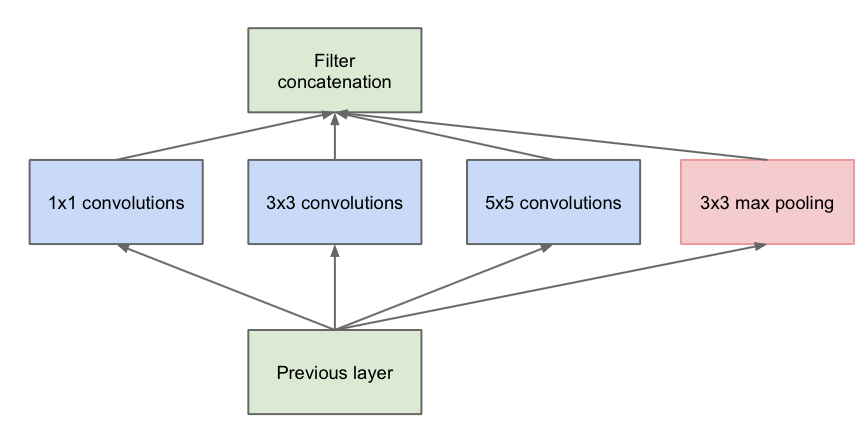
\includegraphics[width=0.8\linewidth]{Pic/18.jpg}
	\end{center}
	\caption{Original inception v1 network}
	 \label{fig:lojbknmng}
	\label{fig:onecol}
\end{figure}

\begin{figure}[t]
	\begin{center}
		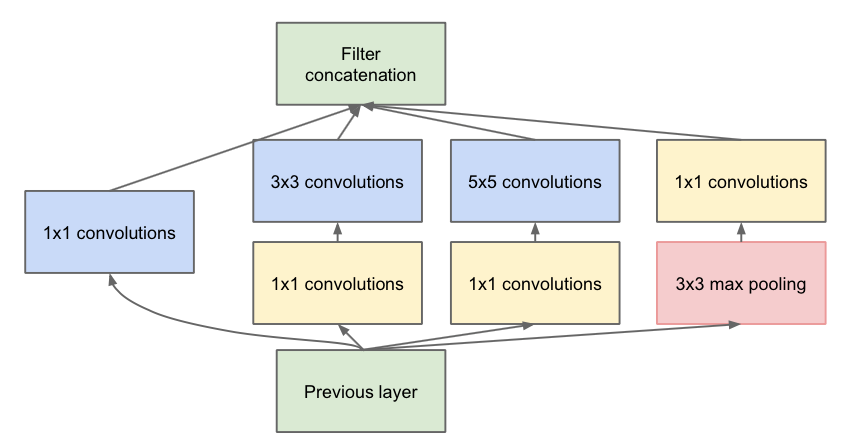
\includegraphics[width=0.8\linewidth]{Pic/19.jpg}
	\end{center}
	\caption{Advanced inception v1 network}
	 \label{fig:long}
	\label{fig:onecol}
\end{figure} 

Because Inception v1 has 5*5 kernels which means 25 parameters, so in this article\cite{ioffe2015batch}, the author try to use two 3*3 kernels to replace the 5*5 kernel, which can reduce number of parameters and accelerate calculation. Inception v2 have batch normalization layer, which reduces internal covariate shift and normalized the output of each layer to an standard normal distribution.

\begin{figure}[t]
	\begin{center}
		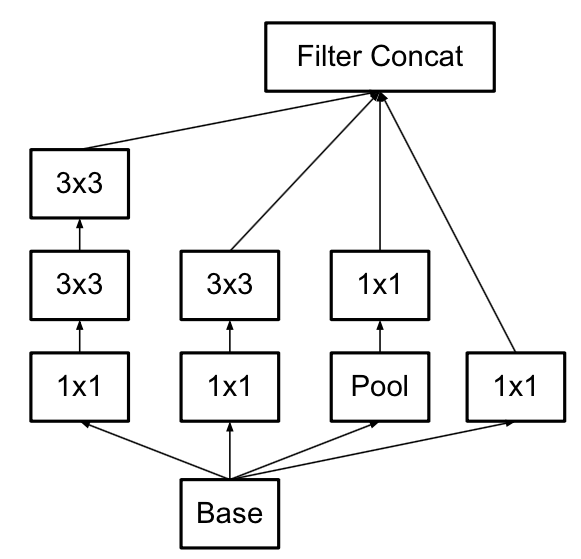
\includegraphics[width=0.8\linewidth]{Pic/16.jpg}
	\end{center}
	\caption{Difference between inception v2 and inception v1} \label{fig:long}
	\label{fig:onecol}
\end{figure}

One of the most important improvements to inception v3 is factorization, which decomposes 7x7 into two one-dimensional convolutions (1x7, 7x1) and so do 3x3 (1x3, 3x1). This method can speeding up calculations (so we can use excess calculations capability to deepen the network), and can also split a conv into two convs, which further increases the depth of the network and increases the nonlinearity of the network. It is also worth noting that the network input has changed from 224x224 to 299x299. 35x35/17x17/8x8 modules are designed.\cite{szegedy2016rethinking}

\begin{figure}[t]
	\begin{center}
		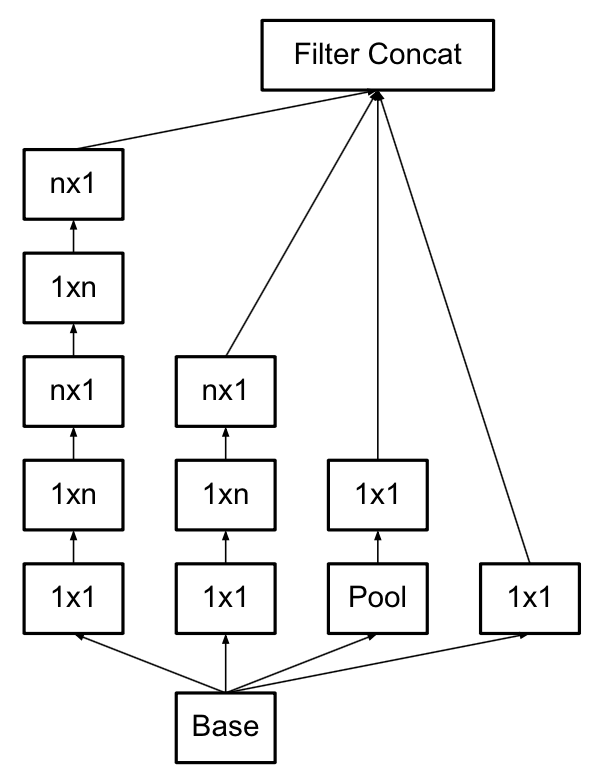
\includegraphics[width=0.8\linewidth]{Pic/17.jpg}
	\end{center}
	\caption{Difference between inception v3 and inception v2} \label{fig:long}
	\label{fig:onecol}
\end{figure}

After Resnet v1 has been proposed, the google team find that the structure of Resnet can greatly speed up the training and improve performance at the same time. So they introduced the residual structure based on the inception v3, proposed the inception-resnet-v1 and inception-resnet-v2, and modified the inception module to propose an inception v4 structure\cite{szegedy2016inception-v4}. The inception-v4 network has become deeper than v3. Before the GAP Inception-v3 includes four convolutional module operations (one regular convolution block and three inception structures), and Inception-v4 has a six convolutional module. Comparing the number of convolution kernels of both, Inception-v4 also has a lot more increase than Inception-v3.

Experiments based on inception v4 have found that similar results to the inception-resnet-v2 structure can be achieved without introducing a residual structure.So they combine the structure of Inception  get an Inception-ResNet v2 network, and also design a deeper and more optimized Inception v4 model that can achieve performance comparable to Inception-ResNet v2.




\begin{figure}[htbp]
	\centering
	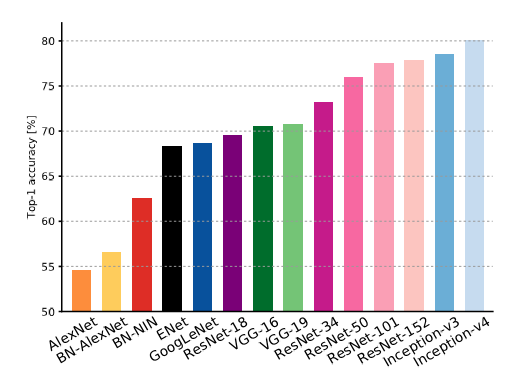
\includegraphics[width=0.8\linewidth]{Pic/16.png}
	\caption{Single-crop top-1 validation accuracies for top scoring single-model architectures.  We introduce with this chart our choice of
		colour  scheme,  which  will  be  used  throughout  this
		publication to distinguish effectively different archi-
		tectures and their correspondent authors.  Notice that
		networks of the same group share the same hue, for
		example ResNet are all variations of pink.}\label{fig:dkhgigit}
\end{figure}

Figure\ref{fig:dkhgigit}, in \cite{canziani2016an} shows the result that Top1 error vs the  network. In the $x-axis$ ,we can see that the different types of the network. The accuracy get more and more accurate.The accuracy increase to about $80\%$ from lower than $55\%$. 


\begin{figure}[htbp]
	\centering
	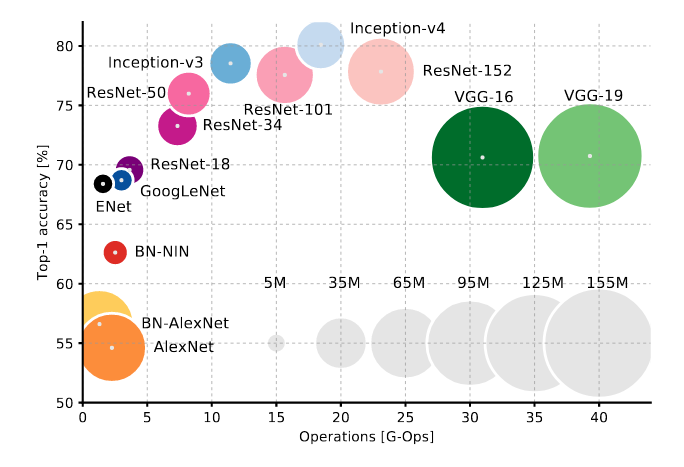
\includegraphics[width=0.8\linewidth]{Pic/17.png}
	\caption{Top 1 vs operations ,size $\infty$ parameters }\label{fig:dkgmhhgigit}
\end{figure}



Top-1 one-crop accuracy versus amount of operations
required for a single forward pass.   The size of the
blobs is proportional to the number of network pa-
rameters; a legend is reported in the bottom right cor-
ner, spanning fromparams. Both these figures share the same
y-axis, and the grey dots  highlight the centre of the blobs
Figure\ref{fig:dkgmhhgigit} shows the result that accuracy different size of 
the models. The larger the model, the big the radius.

\begin{figure}[htbp]
	\centering
	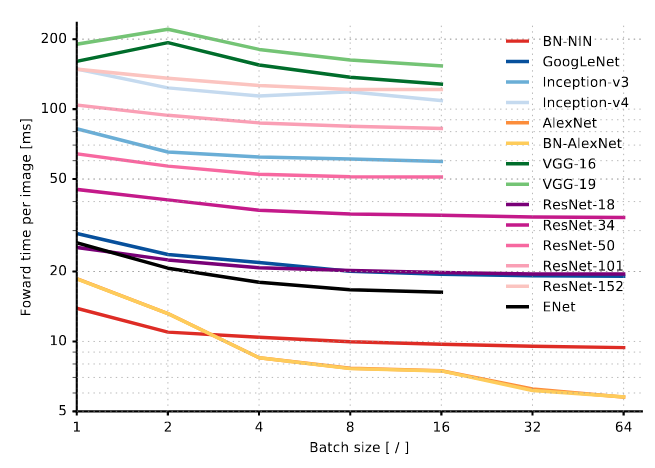
\includegraphics[width=0.8\linewidth]{Pic/18.png}
	\caption{Top 1 vs operations ,size $\infty$ parameters }\label{fig:dkgmjklvhhgigit}
\end{figure}

Figure\ref{fig:dkgmjklvhhgigit}  in \cite{canziani2016an} shows the result that reference image. For each image that the VGG-NET need to take about $200ms$, This is because that the it is very large and there are a lot of parameters in it.


\begin{figure}[htbp]
\centering
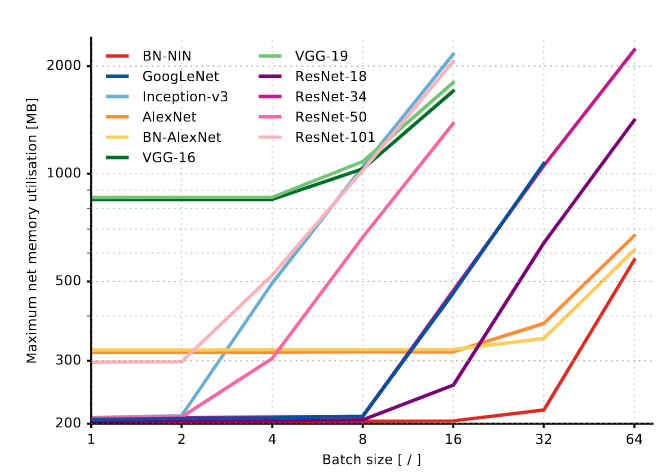
\includegraphics[width=0.8\linewidth]{Pic/19.png}

\caption{memory vs batch size }

\label{fig:dkgmvfghgghjigit}

\end{figure}

Figure in \ref{fig:dkgmvfghgghjigit} in \cite{canziani2016an}, shows the the memory vs the batch size ,from the image we can see different size of the memory need for each model. Different model need different memorize at the initial point.With the batch size increases the memory increases. 



\begin{figure}[htbp]
	\centering
	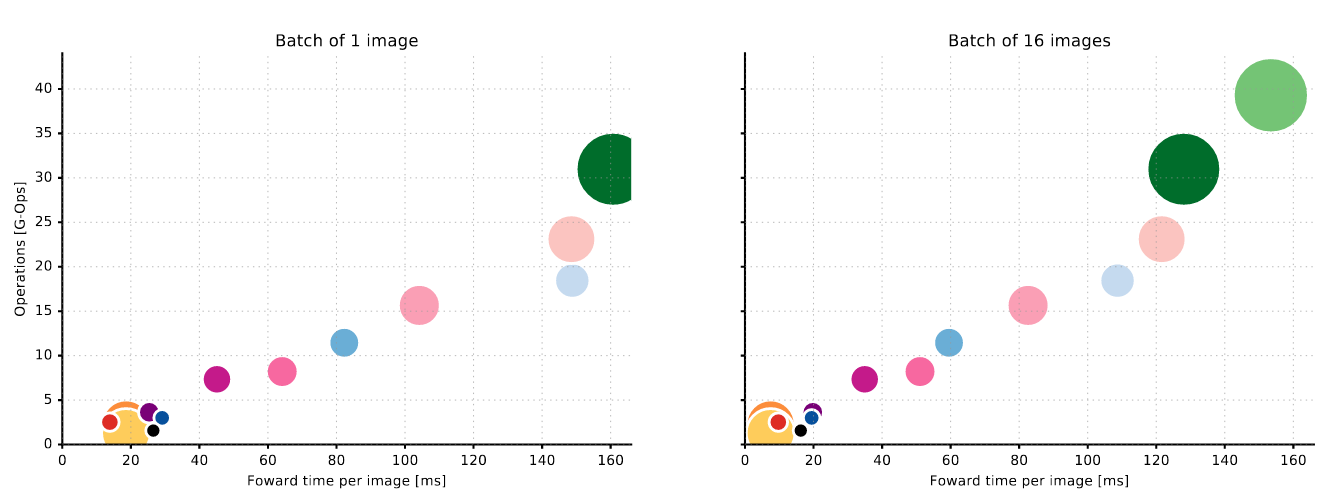
\includegraphics[width=0.8\linewidth]{Pic/20.png}
	
	\caption{Operations	vs inference time ,size$\infty$	parameters.Relationship between operations and inference
		time, for batches of size 1 and 16 (biggest size for which all architectures can still run).  Not surprisingly, we
		notice a linear trend, and therefore operations count represent a good estimation of inference time. Furthermore,
		we can notice an increase in the slope of the trend for larger batches, which correspond to shorter inference
		time due to batch processing optimisation.}
	
	\label{fig:dkgmvfghghgghjigit}
	
\end{figure}



Figure \ref{fig:dkgmvfghghgghjigit} in \cite{canziani2016an} shows the result that the operations with the inference time the operations is very large, the inference time is longer.








\section{CNN based Medical Image Classification}

%-------------------------------------------------------------------------
\subsection{Introduction}

Convolutional neural networks (CNNs) have been used in the field of computer vision for decades. However, their true value had not been discovered until the ImageNet competition in 2012, a success that brought about a revolution through the efficient use of graphics processing units (GPUs), rectified linear units, new dropout regularization, and effective data augmentation. Acknowledged as one of the top 10 breakthroughs of 2013, CNNs have once again become a popular learning machine, now not only within the computer vision community but across various applications ranging from natural language processing to hyperspectral image processing and to medical image analysis. The main power of a CNN lies in its deep architecture, which allows for extracting a set of discriminating features at multiple levels of abstraction\cite{tajbakhsh2016convolutional}.

However, training a deep CNN with full training is very complicated. First, CNNs require a large
amount of labeled training data. Second, training a deep CNN requires extensive computational and memory resources, without that the training process would be extremely time-consuming.Third, training a deep CNN is often complicated by overfitting. Therefore, deep learning from scratch can be tedious and time-consuming, demanding a great deal of diligence, patience, and expertise.

In this survey, I conducted an extensive set of experiments for 4 medical imaging applications: 1) polyp detection in colonoscopy videos~\cite{ribeiro2016colonic}\cite{zhang2017automatic}, 2) image quality assessment and classification in tissues and cells such as blood vessels videos\cite{mcilroy2017vivo}\cite{li2017cell}\cite{huang2017epithelium}\cite{kieffer2017convolutional}\cite{hadad2017classification}\cite{araujo2017classification}, 3) lung disease such as pulmonary embolism detection and so on in computed tomography (CT) images\cite{shen2015multi}\cite{li2014medical},4) dental disease in X-ray image\cite{prajapaticlassification} and 5) intima-media boundary segmentation in ultrasonographic images\cite{roth2015anatomy}.

\subsection{Polyp Detection}

Colorectal cancer (CRC) is one of the leading causes of deathworldwide with about estimated 700 thousand deaths in 2012\cite{zhang2017automatic}. Long-term follow-up studies confirmed that removal of adenomatous polyps reduces CRC mortality. Colonoscopy is the preferred technique for colon cancer screening and prevention. The goal of colonoscopy is to find and remove colonic polyps—precursors to colon cancer. But polyps can appear with substantial variations in color, shape, and size. The challenging appearance of polyps can often lead to misdetection\cite{ribeiro2016colonic}. Polyp miss-rates are estimated to be about 4\% to 12\%; however, a more recent clinical study is suggestive that this misdetection rate may be as high as 25\%. So nowadays, there are many research groups start to use computer aided method such as CNN.

In the article\cite{ribeiro2016colonic}, the author have a small dataset, which only have 100 images(75 abnormal images and 25 healthy images). After finishing the data augmentation which results in 800 images, they resized the 256*256 image to 128*128. In order to test the five architecture they established, he used cross validation method(56 for training and 6 for testing), the result can be seen in Figure \ref{fig:lnvong}, the accuracy is just 75\% to 80\%.

\begin{figure}[t]
	\begin{center}
		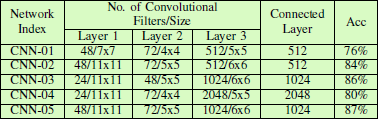
\includegraphics[width=0.8\linewidth]{Pic/4.png}
	\end{center}
	\caption{Accuracy results from different CNN configurations}
	\label{fig:lnvong}

\end{figure}

In order to improve the accuracy, in the evaluation phase, the author obtained the final decision for a 256*256 pixel image by majority voting of the decisions of all 128*128 pixel subimages(patches). This is a kind of fine-tuning. The redundancy of overlapping subimages can increase the system accuracy likewise to give the assurance of certainty for the overall decision. The result can be seen in figure \ref{fig:loghmkng}. They also perform a random patch extraction and it can be concluded that there is not much difference between 16384 subimages or
just 32 subimages (accuracy of 90.96\%), saving considerable computation time and achieving good results.

\begin{figure}[t]
	\begin{center}
		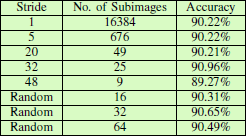
\includegraphics[width=0.8\linewidth]{Pic/5.png}
	\end{center}
	\caption{Accuracy of different strides for overlapping subimages in the evaluation.}
	\label{fig:loghmkng}

\end{figure}

In the second article\cite{zhang2017automatic}, the author use a small datasets(PHW Database), this dataset consisted of 1104, 263 and
563 images without polyps, with hyperplasia polyps and adenomatous polyps, respectively, taken under either WL or NBI endoscopy. For fair comparison, 50 images from each class (nonpolyp, hyperplasia, and adenoma) were randomly selected as testing dataset, while the rest were treated as training dataset.

Because this dataset has an imbalanced number of images for each class, Previous study for polyp detection proposed to use an up/down sampling strategy to tackle such challenge. In this paper, the authors randomly down sampled the majority class to match the sample size of the minority class for both target tasks. The source dataset used ILSVRC and Places205 and trained for 450 000 iterations. They tested two tasks using this database, first is polyp detection and second polyp type classification. In order to do the evaluation, the authors used a feature engineering technique: bag-of-words for comparison. After finishing these tasks, we can see the results in the Figure \ref{fig:lofghmng},\ref{fig:lonmng},\ref{fig:longbng}. In these figures, we can see that transferring low-level CNN features gives better transfer learning performance for both target tasks and when a CNN structure is directly
used for detection and classification. The performance of the proposed method is better in both tasks.

\begin{figure}[t]
	\begin{center}
		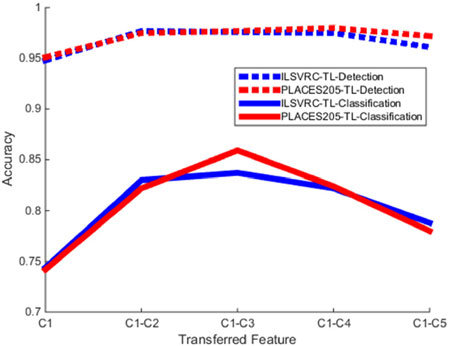
\includegraphics[width=0.8\linewidth]{Pic/6.jpg}
	\end{center}
	\caption{Average accuracy of the detection and classification tasks by transferring C1–Cn features learned from ILSVRC and Places205 and using SVM as the classifier with a RBF kernel.}
	\label{fig:lofghmng}

\end{figure}

\begin{figure}[t]
	\begin{center}
		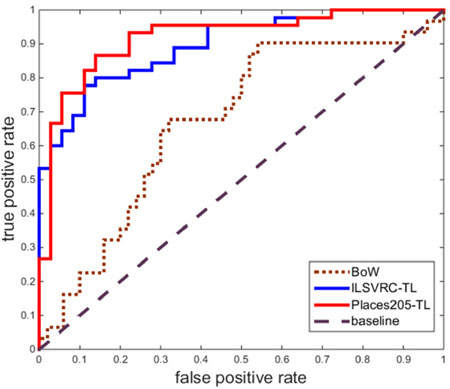
\includegraphics[width=0.8\linewidth]{Pic/7.jpg}
	\end{center}
	\caption{Typical ROC curve for polyp classification for PWH database.}
	\label{fig:lonmng}

\end{figure}

\begin{figure}[t]
	\begin{center}
		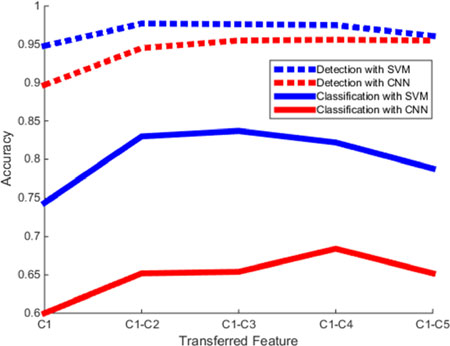
\includegraphics[width=0.8\linewidth]{Pic/8.jpg}
	\end{center}
	\caption{Average accuracy of the detection and classification tasks by transferring C1–Cn features learned from ILSVRC and using either RBF kernel SVM or a fully connected CNN layer with a softmax classifier}
	\label{fig:longbng}

\end{figure}

\subsection{Tissue Detection and Classification}

In this part, I will choose two typical article to discuss. In the first article\cite{kieffer2017convolutional}, the author used feature vectors from several pre-trained structures, including networks with/without transfer learning to evaluate the performance of pre-trained deep features versus CNNs which have been trained by that specific dataset as well as the impact of transfer learning with a small number of samples. This experiment is done on Kimia Path24 dataset which consists of 27,055 histopathology training patches in 24 tissue texture classes along with 1,325 test patches for evaluation. In order to do this experiment, the author used fine-tuning method and a pre-trained CNN as a feature extractor and a fine-tuned CNN as a classifier.

\begin{figure}[t]
	\begin{center}
		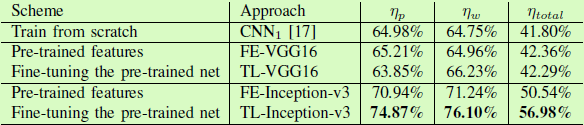
\includegraphics[width=0.8\linewidth]{Pic/12.png}
	\end{center}
	\caption{Comparing the results training form scratch , using deep features via a pre-trained network with no change (FE-VGG16), and classification after fine-tuning a pre-trained network (TL-VGG16, TL-Inception-v3). The best scores are highlighted in bold.(\textit{$\eta_p$} means the patch-to-scan accuracy and \textit{$\eta_n$} means whole-scan accuracy)}
	\label{fig:lovhgmjng}

\end{figure}

The result shows in figure \ref{fig:lovhgmjng} that pre-trained networks are quite competitive against training from scratch. In this figure \ref{fig:lovhgmjng}, VGG16 and CNN are quite similar, whereas the results for Inception-v3 are similar with the transfer-learned model outperforming the feature extractor. But considering Inception-v3 requires no extra effort and produces similar results with a linear SVM, one may prefer using it to training from scratch and fine-tuning a pre-trained net.

In the next article\cite{araujo2017classification}, the authors designed a specific CNN network which perform image-wise classification in four classes of medical relevance: normal tissue, benign lesion, in situ carcinoma and invasive carcinoma. The proposed CNN architecture is designed to integrate information from multiple histological scales, including nuclei, nuclei organization and overall structure organization. A data augmentation method is adopted to increase the number of cases in this training set. A SVM classification using the features extracted by the CNN is also used for comparison purposes.

The dataset is composed of an extended training set of 249 images, and a separate test set of 20 images. In these datasets, the four classes are balanced. The images were selected so that the pathology classification can be objectively determined from the image contents. An additional
test set of 16 images is provided with images of increased ambiguity, which they denote as extended dataset.

They first normalized the images. First, the colors of the images are converted to optical density (OD) using a logarithmic transformation. Then, they used singular value decomposition (SVD)  to the OD tuples to find the 2D projections with higher variance. The resulting color space transform is then applied to the original image. Finally, the image histogram is stretched so that the dynamic range covers the lower 90\% of the data.

Then they do two kinds of classification: Image-wise classification and CNN patch-wise classification. Image-wise classification first divided the origin image into twelve contiguous non-overlapping patches and then use one of three different patch patch methods: majority voting, maximum probability and sum of probabilities. CNN patch-wise classification used 75\% of the data to do the training and validated on the remaining images.The validation set is randomly selected for each epoch. The training process stops after the stabilization of the validation accuracy with equal weight for all the classes (50 epochs). The authors also used the features extracted by the CNN to train a SVM classifier to do the comparison. The result can be seen in figure\ref{fig:ldgfhong} ,\ref{fig:loghng}and \ref{fig:lomhng}.

\begin{figure}[t]
	\begin{center}
		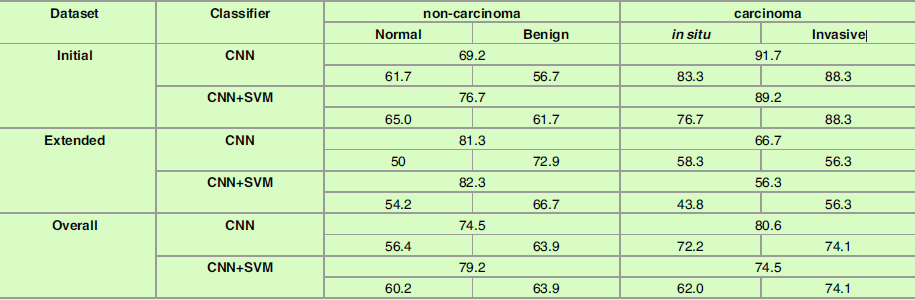
\includegraphics[width=0.8\linewidth]{Pic/13.png}
	\end{center}
	\caption{Patch-wise sensitivity (\%) (2 and 4 classes).}
	\label{fig:ldgfhong}

\end{figure}

\begin{figure}[t]
	\begin{center}
		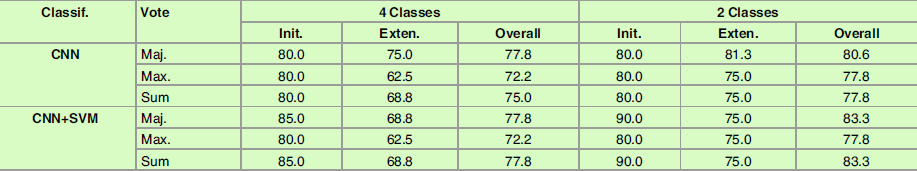
\includegraphics[width=0.8\linewidth]{Pic/15.png}
	\end{center}
	\caption{Image-wise accuracy (\%) using different voting rules (2 and 4 classes).}
	\label{fig:loghng}

\end{figure}

\begin{figure}[t]
	\begin{center}
		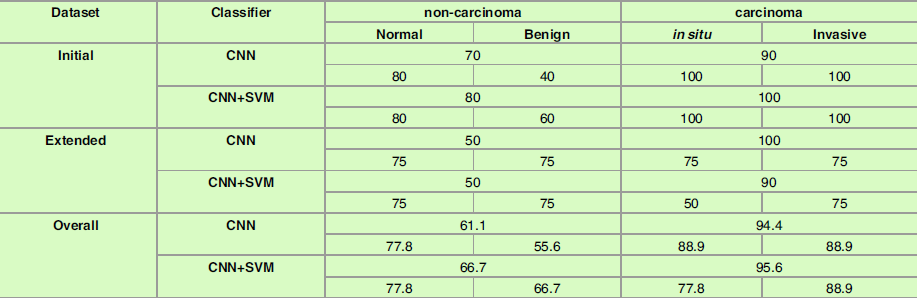
\includegraphics[width=0.8\linewidth]{Pic/14.png}
	\end{center}
	\caption{Image-wise sensitivity (\%) using majority voting (2 and 4 classes).}
	\label{fig:lomhng}

\end{figure}

In figure\ref{fig:ldgfhong}, we can see the result similar between the CNN and CNN+SVM. But the performance of this network is lower for the extended dataset due to its increased complexity. In figure \ref{fig:loghng} and \ref{fig:lomhng}, we can see that CNN+SVM get the best result with the majority voting method. In comparison, CNN's performance is only better for the extended set using majority voting. In addition, we can see that maximum probability is the worst performing method in both methods, which means that this method is not suit in this case.

\subsection{Some kinds of lung Diseases Classification}

Lung cancer is notoriously aggressive with a low long-term survival rate. Quantitative analysis in lung nodules using thoracic Computed Tomography(CT) has been a central focus for early cancer diagnosis, where CT phenotype provides a powerful tool to comprehensively capture nodule characteristics. The importance of diagnostically classifying malignant and benign nodules using CT images is to facilitate radiologists for nodule staging assessment and individual therapeutic planning.\cite{shen2015multi}

In the first article\cite{shen2015multi}, the authors used the LIDC-IDRI datasets, which has 1375 nodule pictures(1100 for training and 275 for testing). In order to improve the speed and accuracy, the authors introduced an Multi-scale Convolutional Neural Networks(MCNN) model to do the lung nodule diagnostic classification. This CNN model take multi-scale raw nodule patches and remove the need of any hand-crafted feature engineering work. This network can also deal with noisy data in nodule CT.

Because of the clinical fact that nodule sizes vary remarkably, this network take patches from different scales(3 layers) as inputs in parallel. The parameter is shared between these layers to reduce parameter. When doing the evaluation task, the result is decided by all the layers. The authors use the HOG and uniform LBP descriptor and SVM and RF classifier to do the classification. The result can be seen in figure \ref{fig:lohj,ng} and figure \ref{fig:lofhgtng}. In figure \ref{fig:lofhgtng}, the \textit{$S_w$} means the size of the cell window for SVM and \textit{$n_{pt}$} means the number of neighbourhood points for LBP.

\begin{figure}[t]
	\begin{center}
		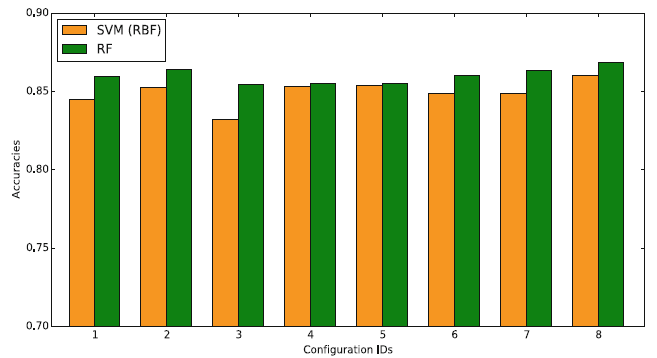
\includegraphics[width=0.8\linewidth]{Pic/9.png}
	\end{center}
	\caption{The classification performance of SVM with the RBF kernel and RF based on features from the MCNN using 8 different configurations. Each configuration is assigned to a unique ID for display convenience}
	\label{fig:lohj,ng}

\end{figure}

\begin{figure}[t]
	\begin{center}
		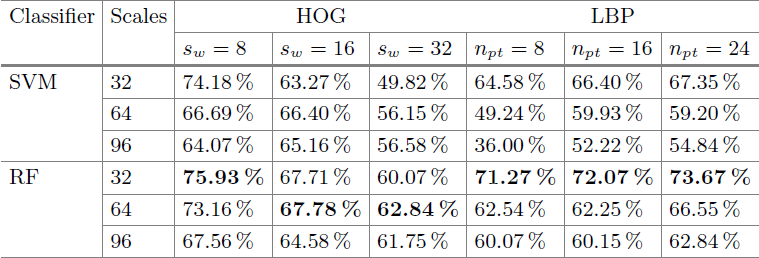
\includegraphics[width=0.8\linewidth]{Pic/10.png}
	\end{center}
	\caption{Performance using the HOG and LBP descriptors with different \textit{$S_w$} and \textit{$n_{pt}$}}
	\label{fig:lofhgtng}

\end{figure}

The second article\cite{li2014medical} is about using CNN to classify the ILD patterns. This experiment used an ILD database which contains 113 sets of HRCT images, with 2062 2D regions indicting the ILD category. In order to augment the dataset, the CT slices were divided into half-overlapping image and the only if 75\% percent of its pixels falling inside the regions of interest will be adopted. The dataset thus contains 16220 image patches from 92 HRCT image sets,
including 4348 norm patches, 1047 emphysema patches, 1953 ground glass patches, 2591 fibrosis patches, and 6281 micronodules patches.

The authors compared their classification results with three other feature extraction approaches: SIFT feature, LBP feature and unsupervised feature learning using RBM. The result can be seen in Figure \ref{fig:lobnmng} . In this figure\ref{fig:lobnmng}, we can see that their customized CNN method achieved the best classification preformance.

\begin{figure}[t]
	\begin{center}
		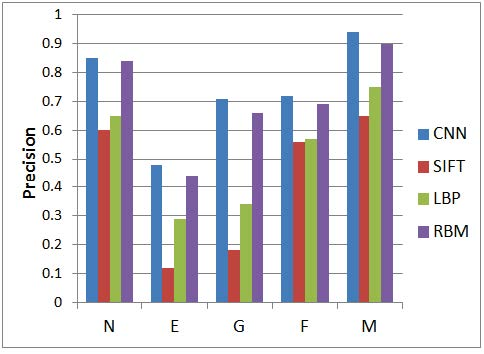
\includegraphics[width=0.8\linewidth]{Pic/11.jpg}
	\end{center}
	\caption{The classification results comparing proposed customized CNN method with SIFT, LBP and RBM}
	\label{fig:lobnmng}
	\label{fig:onecol}
\end{figure}

\subsection{Dental Disease Classification in X-ray Images}

The author found that there is no literature for dental disease classification, so the research group start to use CNN to deal with X-ray images and make some breakthrough. Orthopantomogram (OPG) and Radiovisiography (RVG) x-ray images are the most widely used tools for the diagnoses of dental diseases. Dental caries is one of the most common dental disease worldwide and it has different stages. So the CNN network in this experiment is used to classify mainly 3 classes (dental caries, periapical infection, periodontitis)\cite{prajapaticlassification}.

Because though the radiologists have large dataset of dental x-ray images, these x-ray images have individual privacy issues. So the dataset is very small in this experiment, just have 251 grey images of dimension 1000*1496. So the authors use transfer learning method to do the fine tuning and improve the accuracy very much. They changed some unfrozen layers used for training in order for the pre-trained model to be more adaptive to the training data.

They first resize these picture to 500*748, and then use 180 of 251 to do the training, 45 images for validation and 26 images for testing purpose. Because of the unavailability of the large dataset, CNN architecture could not perform well in this classification task. After they used transfer learning model to do the fine tuning, the accuracy is increased by 15.39\% compared to pure CNN model, and achieved 88.46\% accuracy, which is very encouraging.

\begin{figure}[t]
	\begin{center}
		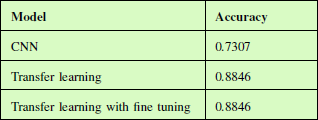
\includegraphics[width=0.8\linewidth]{Pic/2.png}
	\end{center}
	\caption{The comparison of different models}
	\label{fig:long}
	\label{fig:onecol}
\end{figure}

\begin{figure}[t]
	\begin{center}
		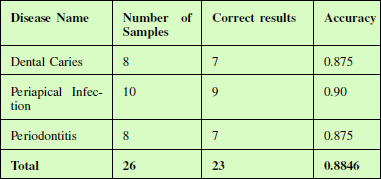
\includegraphics[width=0.8\linewidth]{Pic/3.png}
	\end{center}
	\caption{Experimental results for transfer learning model}
	\label{fig:long}
	\label{fig:onecol}
\end{figure}

\subsection{Intima-media Boundary Segmentation}

Automated classification of human anatomy is an important prerequisite for many computer-aided diagnosis systems. The spatial complexity and variability of anatomy throughout the human body makes classification difficult. So the authors want to use CNN to do this classification. In this paper, the authors choose to use 4298 separate axial 2D key images to learn 5 anatomical classes(neck, lungs, liver, pelvis and legs)\cite{roth2015anatomy}.

When applying the CNN to build the anatomy-specific classifier for CT images, because the authors want to classify these picture to 5 classes, so they choose 5 cascaded layers. All the convolutional filter kernel elements are trained from the data in a supervised fashion. In order to avoid overfitting, the fully-connected layers are constrained, using the \textit{DropOut} method. The datasets are from the Picture Archiving and Communication System (PACS) of the Clinical Center of the National Institutes of Health. In order to enrich their data, they use spatial deformations to each image, using random translation, rotations and non-rigid deformations, which lead their datasets from hundred's picture to near 100 thousand pictures. Before import into the CNN, the author resize all the picture to 256*256 pixels.The authors use 80\% of their total dataset to train the CNN and reserve 20\% to do the test. After doing the experiments, the accuracy of this net can reach 94.1\%, which can be seen in figure \ref{fig:lmnong}.This classification
result is achieved in less than 1 minute on a modern desktop computer and GPU card (Dell Precision T7500,
24GB RAM, NVIDIA Titan Z).

\begin{figure}[t]
	\begin{center}
		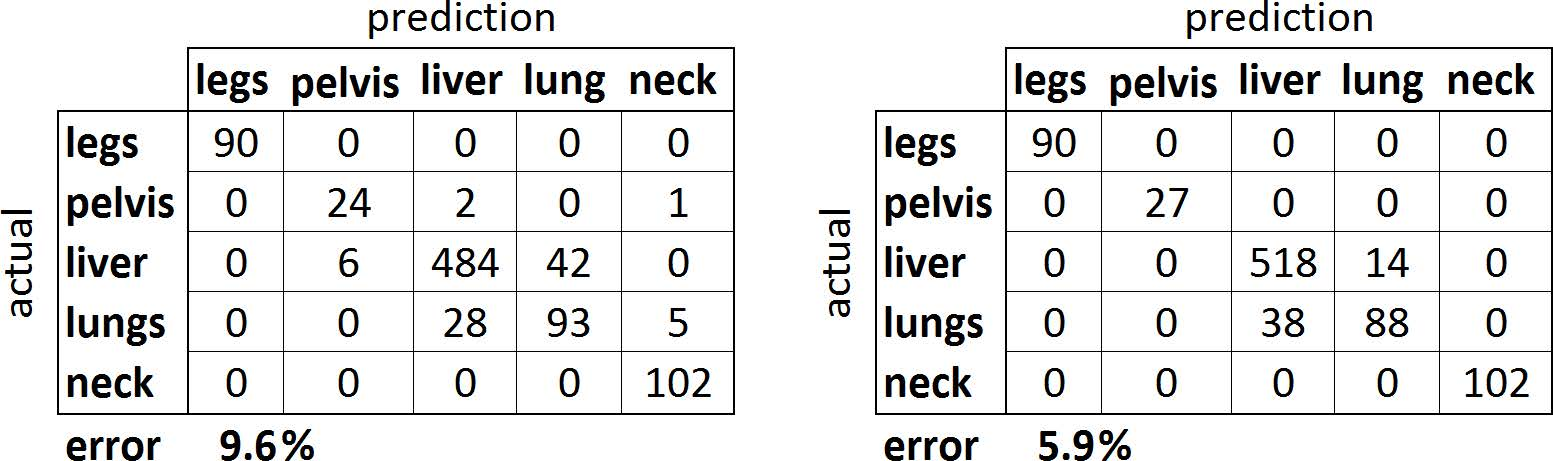
\includegraphics[width=0.8\linewidth]{Pic/1.jpg}
	\end{center}
	\caption{Confusion matrices on the original test images before and after data augmentation.} \label{fig:lmnong}

\end{figure}

\subsection{Conclusion}

In this part, I aimed to address to know how the CNN can be used on the medical image classification and the result these experiments made. My experiment, based on 4 distinct medical imaging applications from different imaging modality systems, have demonstrated that deep CNN are useful for medical image analysis. If the training data is limited, the fine-tuned CNN can perform better than fully trained CNN. I think the potential of CNNs for medical imaging applications is confirmed because both deeply fine-tuned CNNs and fully trained CNNs can outperform the corresponding handcrafted alternatives. We can also see that the speed is depend on the devices, the more powerful the graphics is, the quicker the CNN network use to train.
%\section{Application}

\section{Conclusion}

In this paper we have discussed about the different types of image classification techniques and many CNN based medical application. So this paper will help us in selecting an appropriate classification technique among all the available techniques.


\newpage
{\small
\bibliographystyle{ieee}
\bibliography{egbib}
}

\end{document}
